In this case we aim at finding something even more robust. Even though the Random Forest tree suggested that drawdown information is not as relevant as other features when it comes to predict the future performance of strategies, we decided to give a try to this feature as it is really robust and requires almost no parameter.\\
In detail, the model we try to create here will initially filter as we have seen in the previous two models, but then the remaining strategies will be put in production only if they are somehow showing a steadily growing equity line. In more mathematical terms, what we did is to compute the PnL line for each strategy and each week we see how much time the strategy has spent in drawdown in a certain window in the past. Then we take this number and divide it by the total length of the window. The underlying idea is that if a strategy has spent a lot of time in drawdown it might be that the underlying mean-reversion between traded assets is not working well, or simply it is exposed to significant PnL drops that is something the we really need to avoid. Anyway, the combination between Sharpe-ratio filter and drawdown information might give some additional alpha information to our portfolio construction so we decided to give it a shot. This idea of using drawdown information to forecast the performance of a strategy is not completely new, in fact some articles \cite{challet} invite to use drawdown information as a robust alternative to the Sharpe Ratio. The results for the in-sample gridsearches are as follows: 

\begin{center}
	\centering
	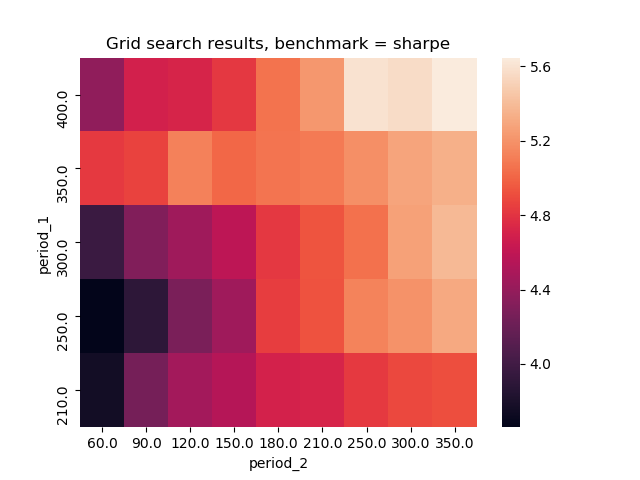
\includegraphics[width=0.6\textwidth]{GridSearches/Average_Drawdown/Figure_1.png}
	\captionof{figure}{GridSearch for the window of Sharpe Ratio and drawdown measure}
	\label{Average_Drawdown_1}
\end{center}

\begin{center}
	\centering
	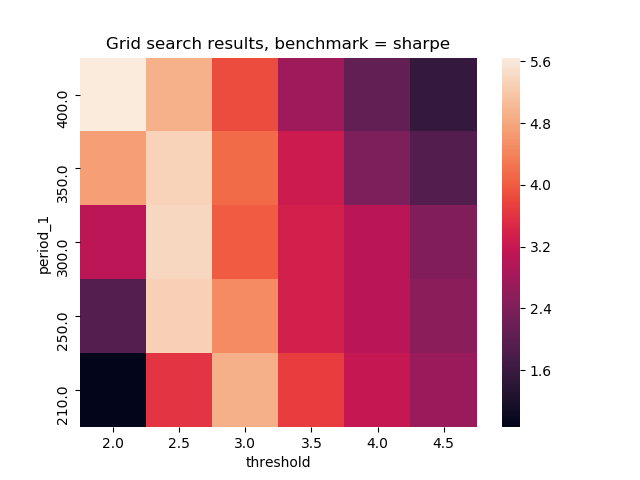
\includegraphics[width=0.6\textwidth]{GridSearches/Average_Drawdown/Figure_2.png}
	\captionof{figure}{GridSearch for the parameters relative to the Sharpe Ratio}
	\label{Average_Drawdown_2}
\end{center}

\begin{center}
	\centering
	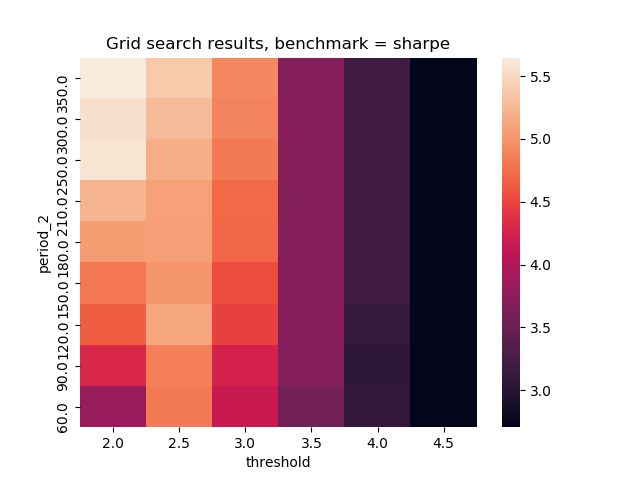
\includegraphics[width=0.6\textwidth]{GridSearches/Average_Drawdown/Figure_3.png}
	\captionof{figure}{GridSearch for drawdown window and sharpe threshold}
	\label{Average_Drawdown_3}
\end{center}

The optimal parameters are close to the ones we have seen for the second method, so we stick with them a part for the ranking period that is a bit longer in this case. Here you can see the resulting equity line:

\begin{center}
	\centering
	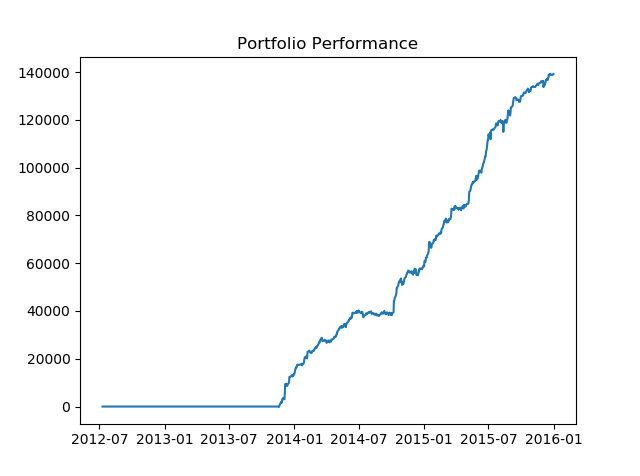
\includegraphics[width=0.6\textwidth]{GridSearches/Average_Drawdown/Average_Drawdown_In_Sample_Performance.png}
	\captionof{figure}{In-Sample performance for the Average-Drawdown method.}
	\label{Average_Drawdown_in_sample}
\end{center}

The statistics are the following:

\begin{table}
	\centering
	\begin{tabular}{c|c}
		\textbf{Statistic} & \textbf{Value} \\\hline
		Sharpe Ratio & 5.1853 \\ 
		Sortino Ratio & 7.7506 \\ 
		Omega Ratio & 2.81 \\ 
		Skewness & 0.8184 \\ 
		Kurtosis & 7.5674 \\ 
		Maximum Drawdown (\% duration/duration) & 12.7 \\ 
		Longest Drawdown (days) & 70.0 \\ 
		Winning Days & 64.557 \\ 
	\end{tabular}
	\caption{\label{tab:widgets} Statistics for the in-sample performance of the Average-Drawdown method.}
\end{table}

The performance is definitely better than that of a plain sharpe-based method, it seems like if we use more precise and/or cleaner information. Therefore our Sharpe ratio increases by 2 units in terms of performance that is really good. 